% !TEX root = ../main.tex

% 报告主体


%---------------------------------------------------------------------
% 实验
\clearpage
\ysySection{实验}

\subsection{采用的是流萤主题}

如\cref{fig:liuyintheme}所示，相应的Python绘图工具也更新了流萤主题。

\begin{figure}[h!]
	\centering
	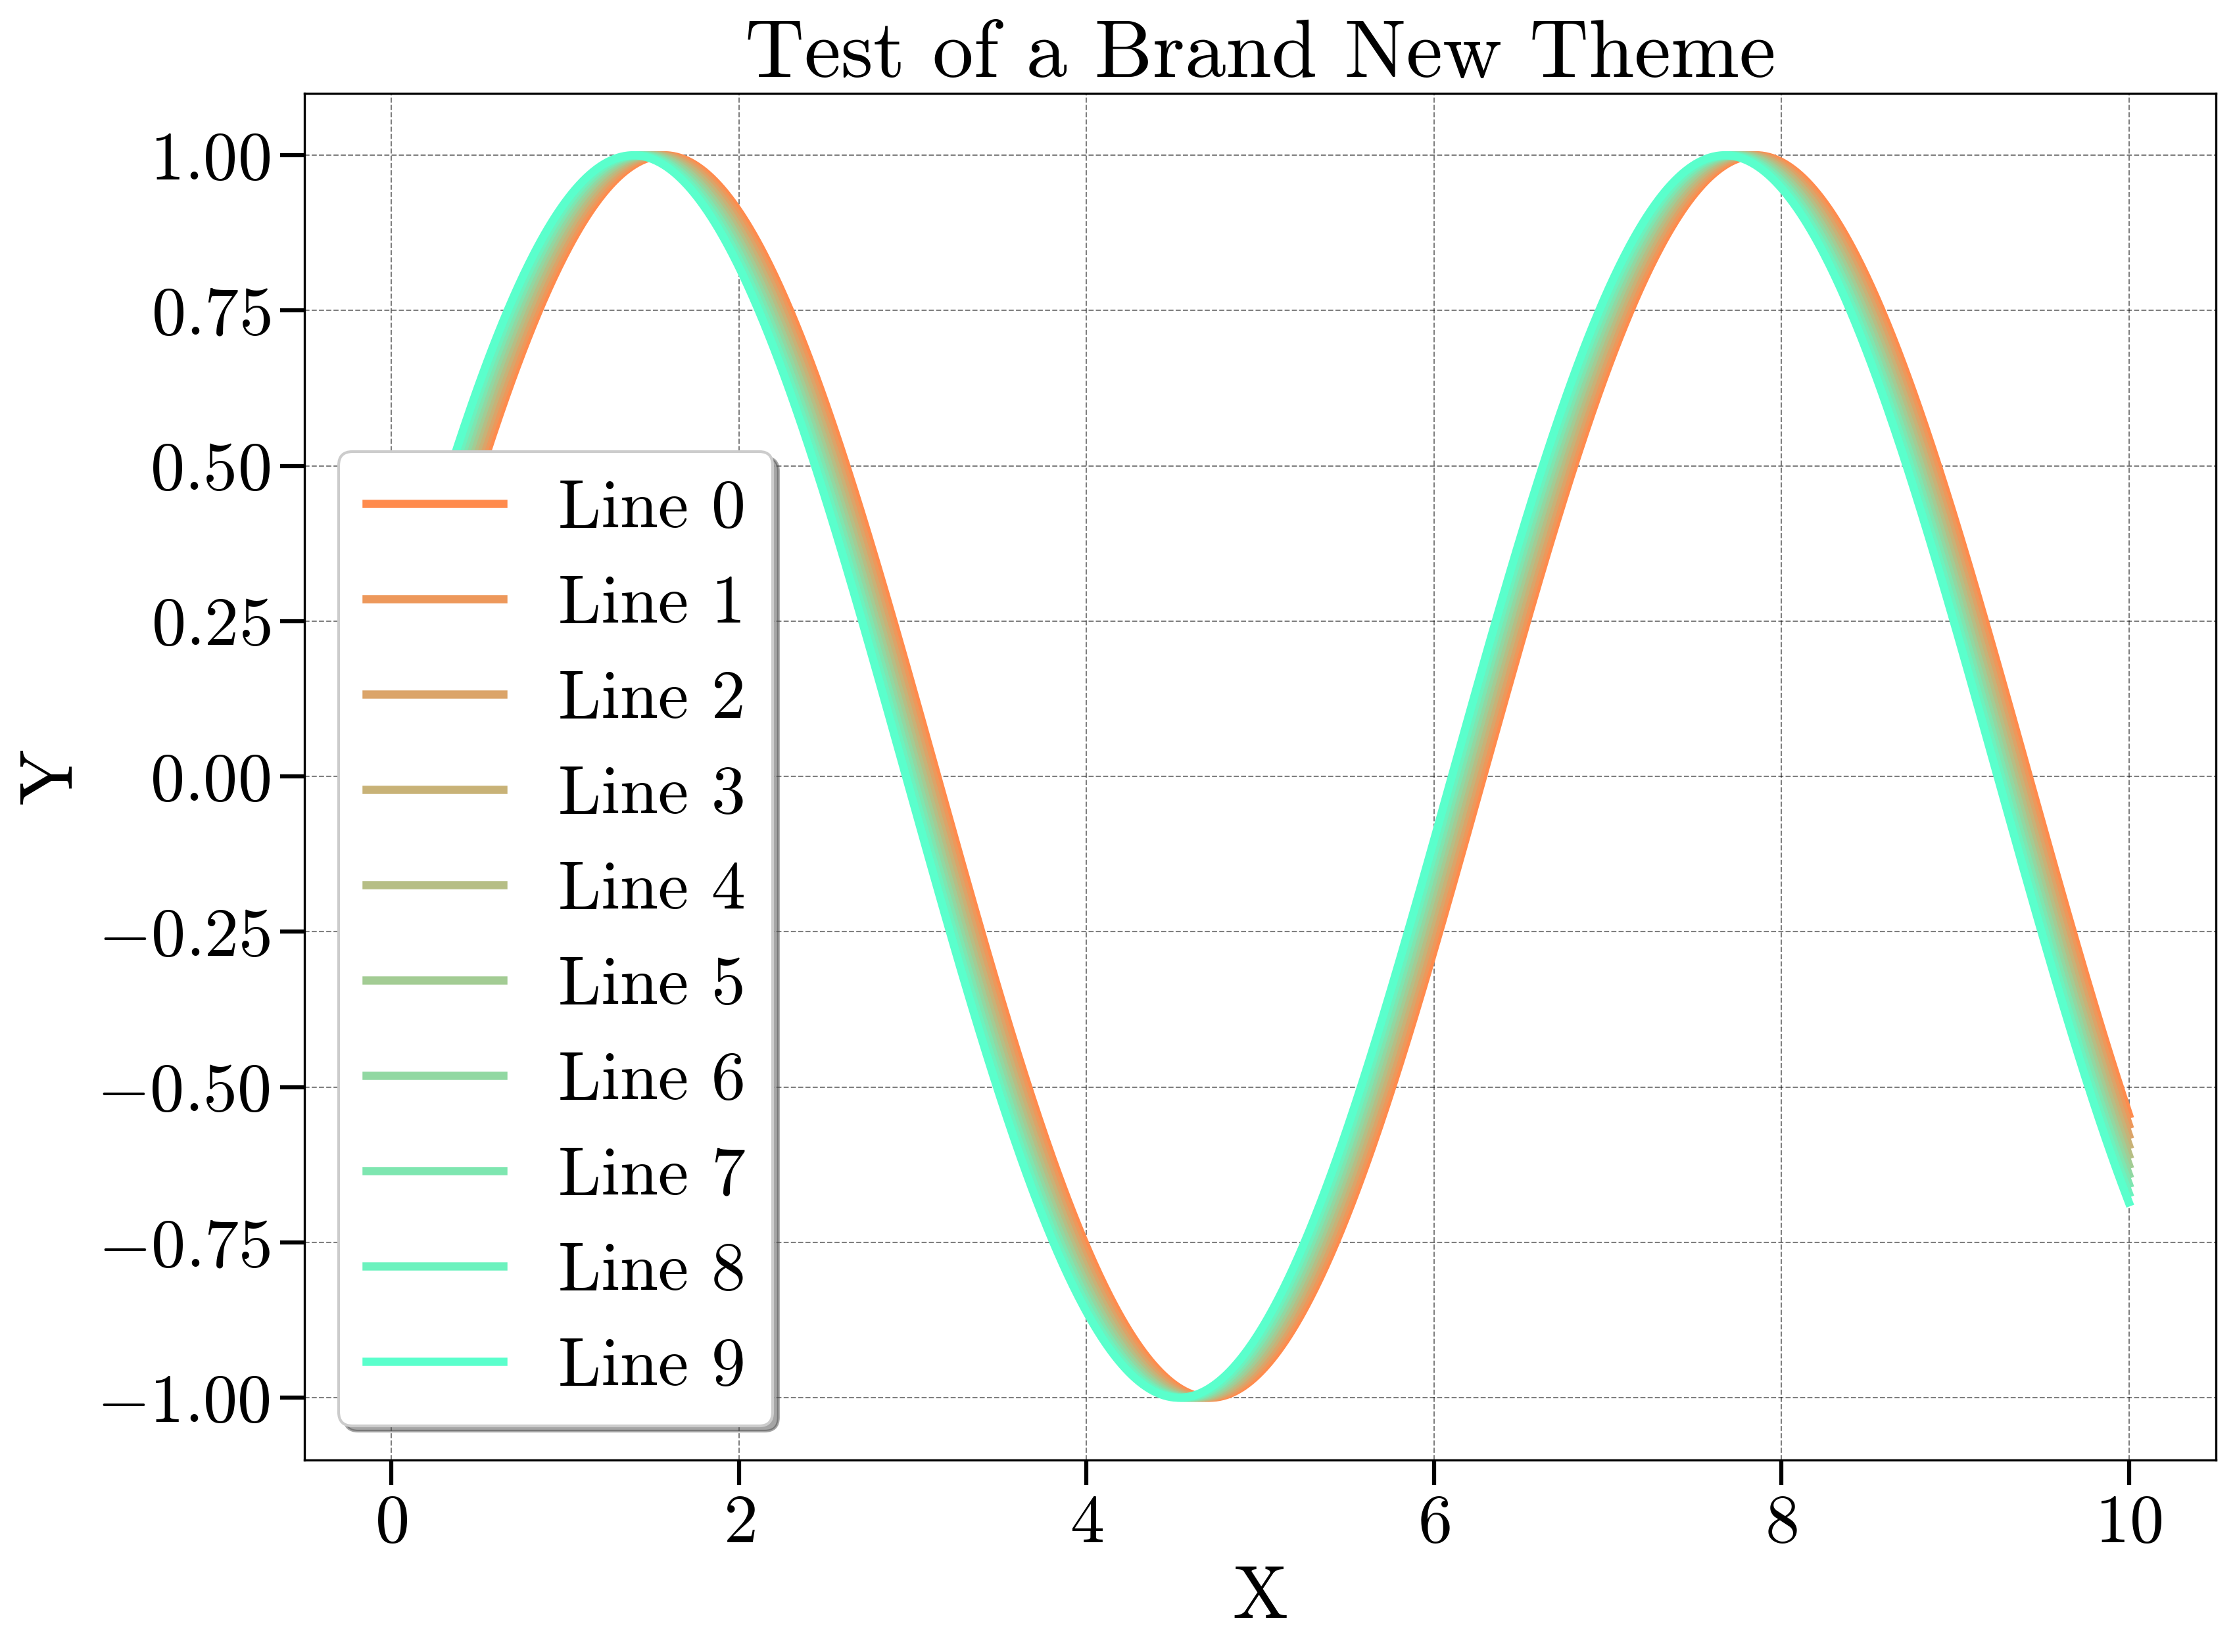
\includegraphics[width=0.9\linewidth]{images/liuyin_theme}
	\caption{我将，点燃星海！}
	\label{fig:liuyintheme}
\end{figure}

同时还更新了数据点的绘制功能（如\cref{fig:displacement}）。

\begin{figure}[h!]
	\centering
	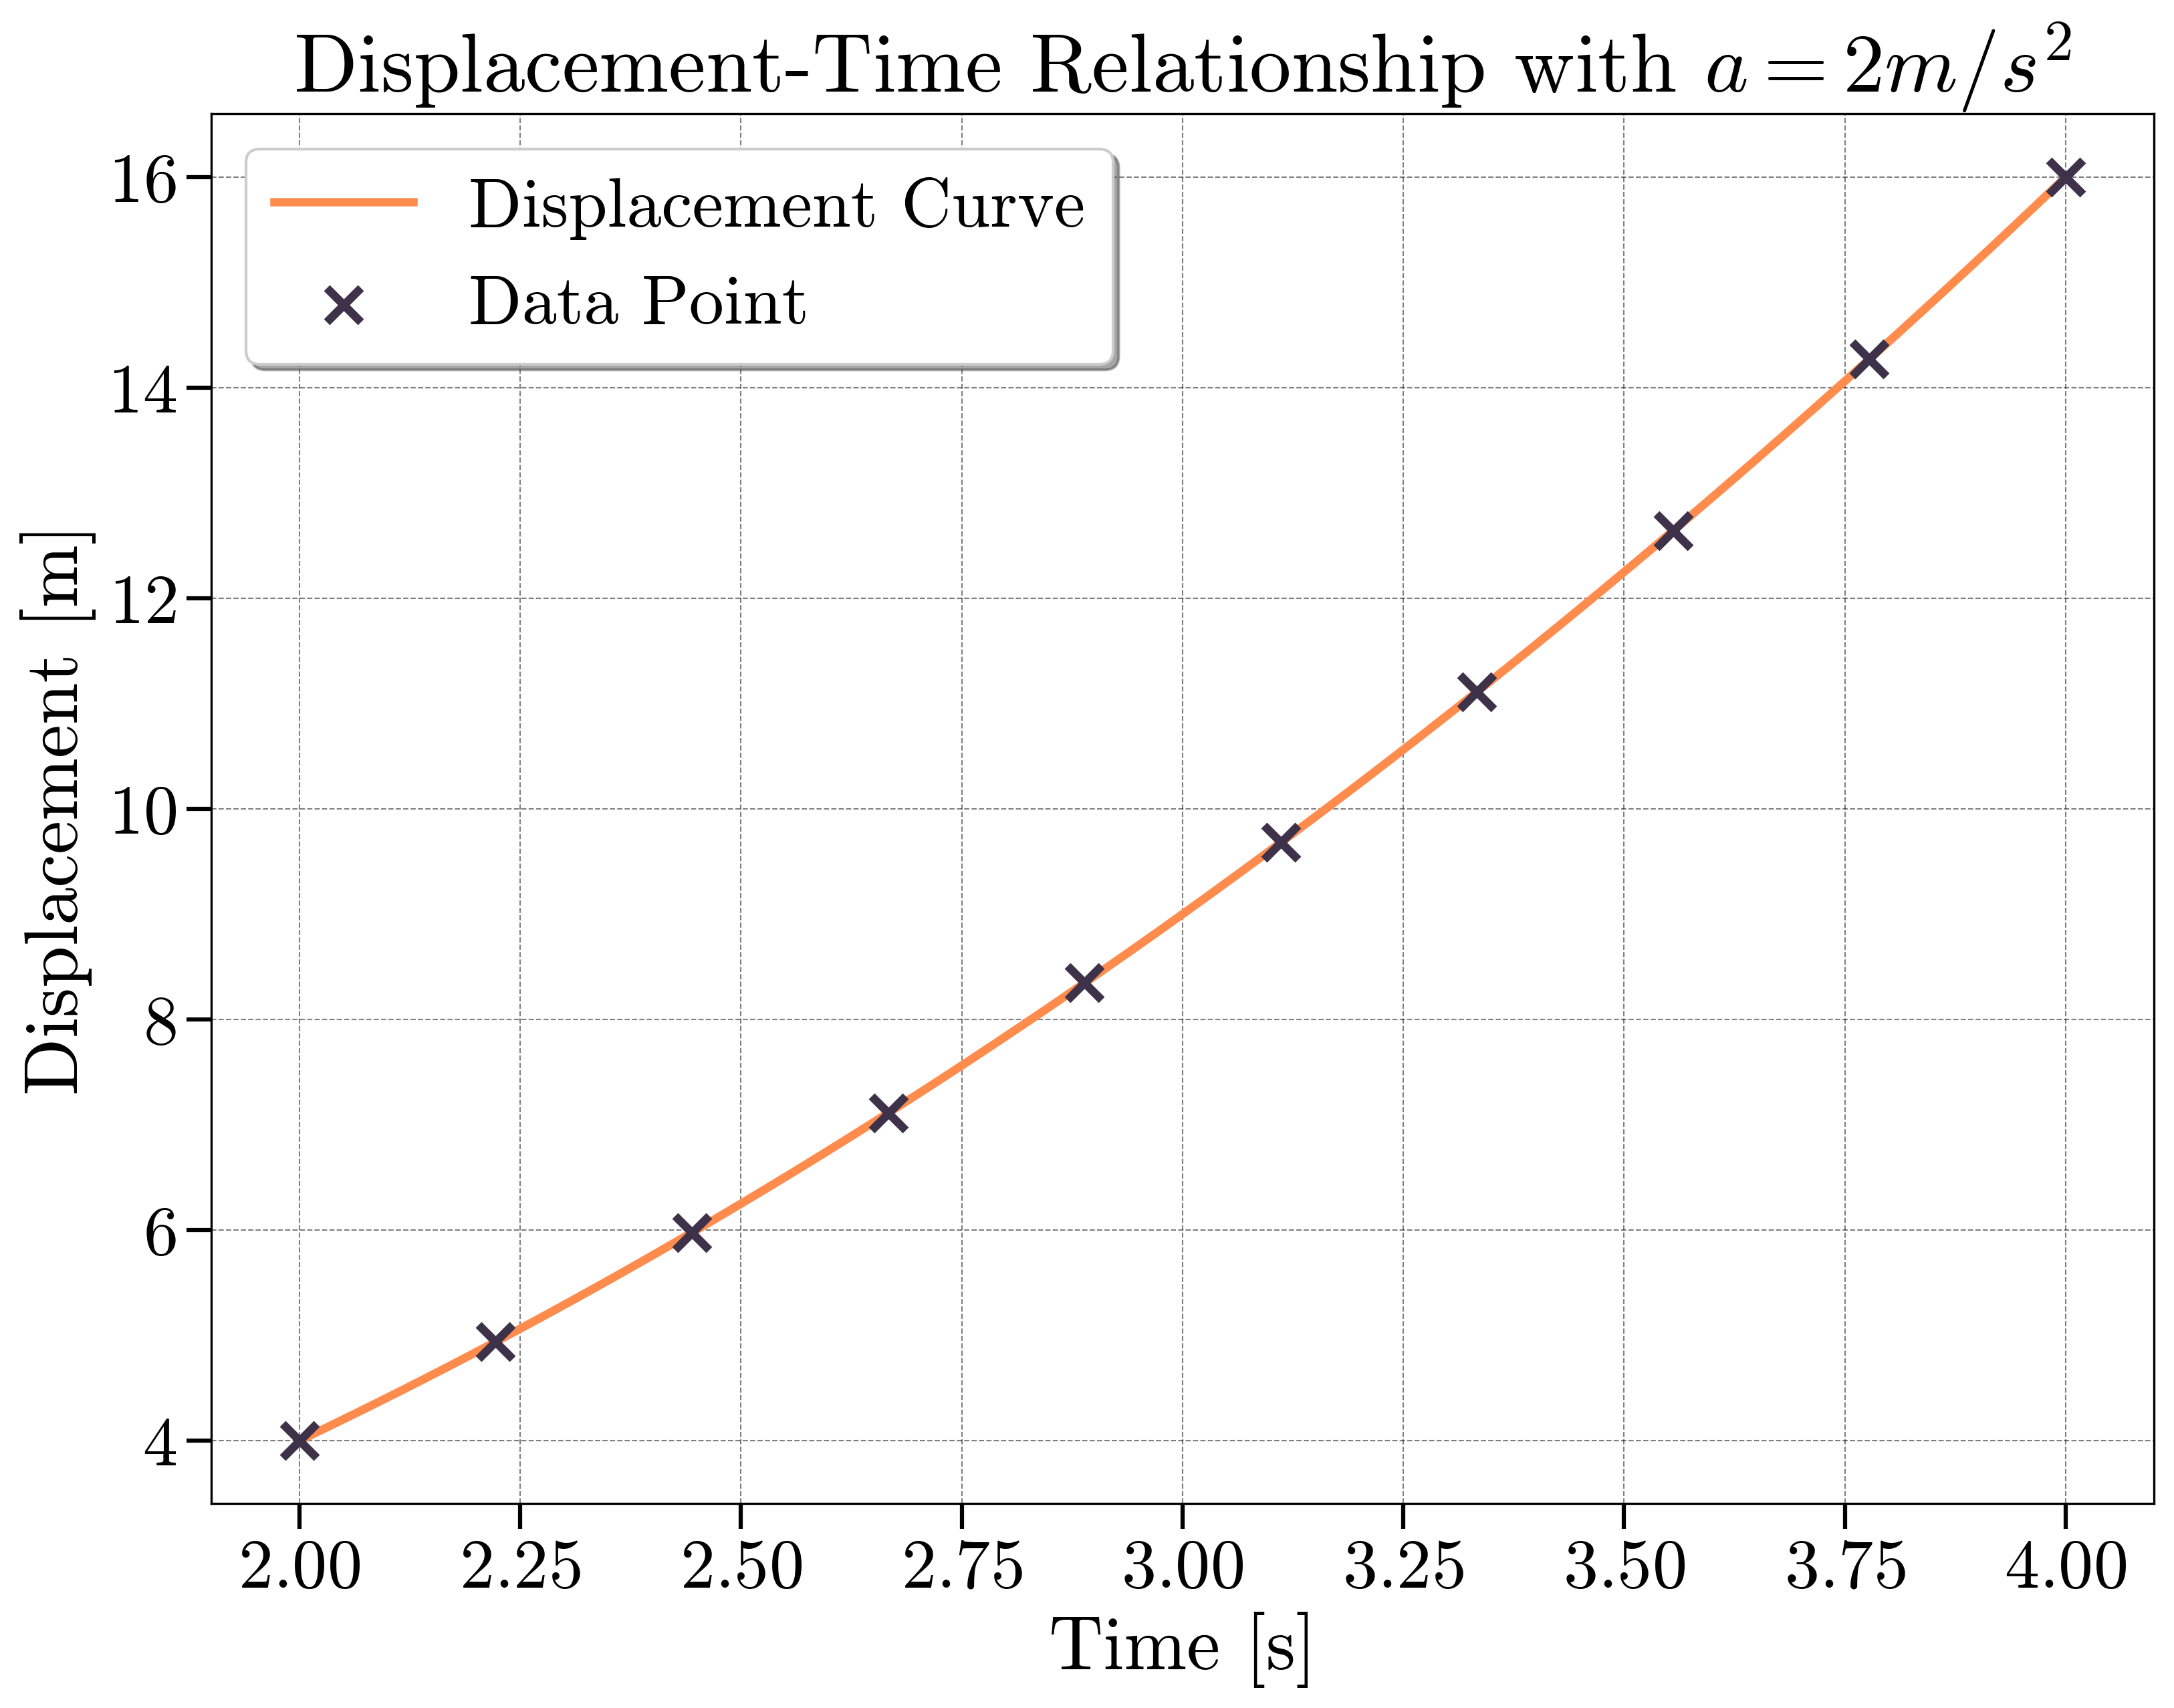
\includegraphics[width=0.7\linewidth]{images/displacement}
	\caption{这是位移-时间关系图}
	\label{fig:displacement}
\end{figure}

\subsection{此外，我还更新了流萤主题的无序列表}

\begin{itemize}
	\item 这是一级；
	\begin{itemize}
		\item 这是二级；
		\begin{itemize}
			\item 这是三级；
			\item 好了，\highlight{别再往下一级了}，下面就没有主题化了。
		\end{itemize}
		
		\item 此外，封面插图我准备了好几幅，可以使得每篇实验报告不重样。
	\end{itemize}
	
	\item 如果你仔细看页眉，你也可以发现流萤的图标。\ysyEmph{现在没有了，我换到了标题上。}
\end{itemize}

%---------------------------------------------------------------------
% 分析与讨论
\ysySection{分析与讨论}

\subsection{分析}

通过计算噪声强度，对电阻热噪声测量值的输入带宽修正、扣除本底和噪声功率谱密度计算最终实现玻尔兹曼常量计算（计算代码见\textbf{附件}）。

\begin{table}[h!]
	\centering
	\renewcommand{\arraystretch}{1.5} % 调整行高
	\caption{本地测量与遥测测量的 $k_B$ 值（单位：J/K）}
	\label{tab:kbvalues}
	\begin{tabular}{|cc|cc|}
		\hline
		\textbf{数据名} & \textbf{本地测量列 $k_B$ (local)} & \textbf{数据名} & \textbf{遥测测量列 $k_B$ (remote)} \\ \hline
		local/Data1 & $1.12\times10^{-23}$ & remote/Data2 & $1.72\times10^{-23}$ \\ 
		local/Data2 & $1.42\times10^{-23}$ & remote/Data3 & $1.35\times10^{-23}$ \\ 
		local/Data3 & $1.38\times10^{-23}$ & remote/Data4 & $1.35\times10^{-23}$ \\ 
		local/Data4 & $1.43\times10^{-23}$ & remote/Data5 & $1.43\times10^{-23}$ \\ 
		local/Data5 & $7.65\times10^{-24}$ & remote/Data6 & $1.35\times10^{-23}$ \\ 
		local/Data6 & $1.47\times10^{-23}$ & remote/Data7 & $1.88\times10^{-23}$ \\ 
		local/Data7 & $2.61\times10^{-23}$ & remote/Data8 & $1.62\times10^{-23}$ \\ 
		local/Data8 & $1.70\times10^{-23}$ & remote/Data9 & $1.42\times10^{-23}$ \\ \hline
	\end{tabular}
\end{table}

\subsection{讨论}

\begin{ubox}{$R(t)$与时间常数和陡降有何关系？}
	在保持陡降不变的前提下，随着时间常数从 30 μs 增加到 1 ms，信号的变化幅度逐渐减小。这是因为较大的时间常数使低通滤波器的通带变窄，从而抑制了高频成分，使得输出信号对快速变化的输入信号响应变得迟缓。尽管增大时间常数可以提高输出信号的稳定性，但时间常数并非越大越好。针对不同特性的待测信号，选择合适的时间常数至关重要。只有在适当的时间常数下，系统才能在保持响应能力的同时，快速捕捉 \( R(t) \) 随时间的变化，确保信号的真实性和有效性。
	
	当保持时间常数不变，将陡降从 6 dB/oct 提高到 24 dB/oct 时，信号变化的幅度也会略微减小。陡降的增加意味着滤波器对高频噪声的抑制更为显著，但若陡降值设置过高，可能导致滤波器对输入信号的响应变得迟缓，从而影响快速变化信号的捕捉准确性。因此，合理选择陡降值非常关键，以便在有效抑制噪声的同时，确保信号的动态变化得以准确呈现。过高的陡降会降低系统对信号变化的敏感性，从而影响测量结果的准确性。
	
	总体而言，对于变化速率不同的待测信号，需要在时间常数和陡降之间找到最佳平衡，以实现最佳的信号捕捉与处理效果。
\end{ubox}

%---------------------------------------------------------------------
% 总结
\ysySection{总结}

\subsection{第一段废话}
实验“电阻热噪声及玻尔兹曼常量测量”旨在通过测量电阻在不同温度下的热噪声来计算玻尔兹曼常量 \( k_B \)。本实验首先通过锁相放大器精确测量电阻的噪声电压信号，并利用 Johnson-Nyquist 公式将噪声与温度、阻值和带宽联系起来，以便从中提取出 \( k_B \) 的值。

\subsection{第二段废话}
实验中对不同参数（如带宽、频率、时间常数等）进行了优化和修正，力求排除环境噪声及设备本底噪声的影响。例如，采用低温测量方式以抑制环境噪声和非期望的热效应干扰。通过在不同环境下（如液氮冷却或室温）进行测量，验证了噪声电平随温度变化的规律，说明了热噪声与温度呈正相关。数据处理阶段，采用对比本底噪声和热噪声的差异，计算出最终的噪声强度。此外，实验对多个测量数据进行了平均，减小了统计误差，并通过误差传播公式计算了 \( k_B \) 的不确定度。结果表明，实验误差的主要来源是本底噪声的系统误差和设备带宽的限制。最终，通过对测得数据的分析和修正，实验得到了接近理论值的玻尔兹曼常量，并验证了 Johnson-Nyquist 热噪声模型的准确性。

\subsection{一个好玩的东西}

\subsubsection{流萤第一定理}

已知：一个流萤加一个流萤等于两个流萤
$$
\liuyin + \liuyin = 2\liuyin
$$

求证：

\[
\int_0^\infty \frac{\liuyin^{\alpha-1}}{(1 + \liuyin^{2})^{\beta}} \, d\liuyin = \frac{\Gamma\left(\frac{\alpha}{2}\right) \Gamma\left(\beta - \frac{\alpha}{2}\right)}{2^{\alpha - 1} \Gamma(\beta)} \quad \text{for} \quad 0 < \Re(\alpha) < 2\beta
\]


\subsubsection{代码环境展示}

\begin{macbox}{</>Python}
	\begin{lstlisting}[style=pythonstyle]
		# 导入必要的库
		import cgc_function_adjusted as cgcfa
		import cgc_plot as cgcp
		
		# j1=2, j2=2
		j1 = 2
		j2 = 2
		# 生成一个CG类
		cg = cgcfa.CG(j1, j2)
		# 将这个CG类的CG系数表完整生成并存储在一个pandas.DataFrame中
		cgdf = cgcp.cg_table_generator(cg)
		# 绘制它
		cgcp.cg_df_plot(cgdf)
	\end{lstlisting}
\end{macbox}

绘制结果见附表中\cref{fig:cgcexample}
